Στο προηγούμενο κεφάλαιο είδαμε από τι αποτελείται ένα σύνηθες σύστημα ξεκλειδώματος πόρτας πολυκατοικίας/σπιτιού. Στο παρόν κεφάλαιο θα αναλύσουμε τον τρόπο σύνδεσης των εξαρτημάτων (βλ \fullref{sec:hardw}), και τον προγραμματισμό τους ώστε να μπορεί να πυροδοτηθεί ξεκλείδωμα της πόρτας μέσω υπολογιστή.

\section{Προετοιμασία του Raspberry Pi}
	Πρώτο βήμα πριν να γίνει η οποιαδήποτε σύνδεση μεταξύ εξαρτημάτων είναι αναγκαίο να γίνει η εγκατάσταση της τελευταίας έκδοσης του Raspbian Lite στο Raspberry Pi Zero W, καθώς επίσης και να συνδεθεί με το internet. Χρησιμοποιείται η έκδοση Lite έναντι της πλήρης έκδοσης, καθώς δεν χρειάζεται γραφικό περιβάλλον όπως επίσης και τα περισσότερα πακέτα που υπάρχουν προεγκατεστημένα στην πλήρη έκδοση.

	Αφότου γίνει η εγκατάσταση του λειτουργικού συστήματος στην κάρτα MicroSD, μπορεί να γίνει η σύνδεση στο Internet είτε Headlessly (χωρίς, δηλαδή, να χρειαστεί να συνδεθεί οθόνη στο RPi), βάζοντας το αρχείο στο \verb|boot| partition (διαμέρισμα) της κάρτας μνήμης, και εφαρμόζοντας το παρακάτω configuration, μέσα στο αρχείο \verb|wpa_supplicant.conf|\textsuperscript{\cite{rpi_wifi_headless}}:

	\begin{lstlisting}
	network={
		ssid="YOUR_NETWORK_NAME"
		psk="YOUR_PASSWORD"
	}\end{lstlisting} 

	Στο πεδίο \verb|ssid| πρέπει να μπει το όνομα του δικτύου στο οποίο πρόκειται να συνδεθεί το RPi. Στο πεδίο PSK πρέπει να γίνει τοποθέτηση του κλειδιού πρόσβασης του δικτύου. Σε περίπτωση που δεν χρησιμοποιείται κρυπτογραφία στο δίκτυο (δεν προτείνεται καθώς μπορεί να συμβεί υποκλοπή δεδομένων από τρίτους), μπορούμε να εισάγουμε το παρακάτω configuration στο ίδιο αρχείο:

	\begin{lstlisting}
	network={
		ssid="YOUR_NETWORK_NAME"
		key_mgmt=NONE
	}\end{lstlisting} 

	Τέλος, πρέπει να γίνει ενεργοποίηση του SSH Daemon στο Raspbian, προκειμένου να είναι εφικτή η απομακρυσμένη σύνδεση στο RPi, μέσω τοπικού δικτύου. Λόγω κατασκευής δικτύων bot (botnets) από διάφορους κακόβουλους χρήστες προκειμένου να γίνουν επιθέσεις DDOS (Distributed Denial of Service) από συσκευές Internet of Things που χρησιμοποιούν τα προεπιλεγμένα (default) στοιχεία πρόσβασης (Username, Password), προς διάφορους στόχους, από τον Νοέμβριο του 2016 είναι απενεργοποιημένος εξ' αρχής ο SSH Daemon και πρέπει να ενεργοποιηθεί από τον χρήστη, αν τον χρειάζεται \textsuperscript{\cite{raspbian_nov2016_upd}}. Για να γίνει αυτό, πρέπει να δημιουργηθεί ένα άδειο αρχείο με το όνομα \verb|ssh| μέσα στο \verb|boot| partition της κάρτας μνήμης του RPi.

	Αφότου γίνει η πρώτη εκκίνηση του RPi και βεβαιωθεί οτι υπάρχει ενεργή σύνδεση στο διαδίκτυο, πρέπει να γίνει σύνδεση στο Raspberry Pi μέσω SSH (Username: pi, Password: raspberry)\textsuperscript{\cite{default_creds}} και να γίνουν τα ακόλουθα βήματα, προκειμένου να ενημερωθεί πλήρως το Raspbian:

	\subsection{Αλλαγή των προεπιλεγμένων στοιχείων πρόσβασης}
		Όπως αναφέραμε προηγουμένως, προκειμένου να μην υπάρξει στο μέλλον κίνδυνος επίθεσης, πρέπει να γίνει αλλαγή των προεπιλεγμένων στοιχείων πρόσβασης στο Raspbian. Πρέπει να εκτελεστεί η εντολή \verb|passwd|, και να γίνει εισαγωγή ενός νέου κωδικού πρόσβασης. Ο νέος κωδικός, προκειμένου να είναι ασφαλής, πρέπει να αποτελείται από τουλάχιστον 12 χαρακτήρες, να μην περιέχει μέσα ονόματα, ονόματα από μέρη, ή γενικά λέξεις οι οποίες υπάρχουν μέσα σε λεξικά, και τέλος θα πρέπει να περιέχει πεζά γράμματα, κεφαλαία, αριθμούς, και σύμβολα\textsuperscript{\cite{secure_passwords}}.

	\subsection{Ενημέρωση του Raspbian}
		Προκειμένου να εξασφαλιστεί η βέλτιστη λειτουργία και η μέγιστη ασφάλεια στο σύστημα, χρειάζεται να γίνει ενημέρωση των πακέτων του λειτουργικού συστήματος. Πρέπει να γίνει εκτέλεση των επόμενων 2 εντολών\textsuperscript{\cite{raspbian_update}}:

		\begin{lstlisting}[language=bash]
		sudo apt-get update
		sudo apt-get dist-upgrade\end{lstlisting}

	Αφότου γίνει η αλλαγή των προεπιλεγμένων στοιχείων πρόσβασης και η ενημέρωση του συστήματος, πρέπει να απενεργοποιηθεί το σύστημα προκειμένου να συνδεθεί με το Relay. 

\section{Σύνδεση με το Relay}
	Για να γίνει η σύνδεση του Raspberry Pi με το Relay, πρέπει να επιλέξουμε έναν από τους 2 τρόπους σύνδεσης, ανάλογα με το τι Relay Module θα χρησιμοποιηθεί (βλ. \fullref{sub:relay}).

	\subsection{Σύνδεση χωρίς την χρήση Arduino}
		Προκειμένου να γίνει σύνδεση του RPi με το Relay Module, θα χρειαστεί να κολληθούν κεφαλές υποδοχής για Jumper Wires στα GPIO του Raspberry Pi. Μπορούν να χρησιμοποιηθούν είτε Female, είτε Male τύπου Headers, αλλά από αυτό θα εξαρτηθεί τι Jumper Wires θα χρειαστούν για να συνδεθεί το RPi με το Relay Module (Male-Female αν χρησιμοποιηθεί Female Header, Female-Female αν χρησιμοποιηθεί Male Header).

		\begin{figure}[h]
			\centering
				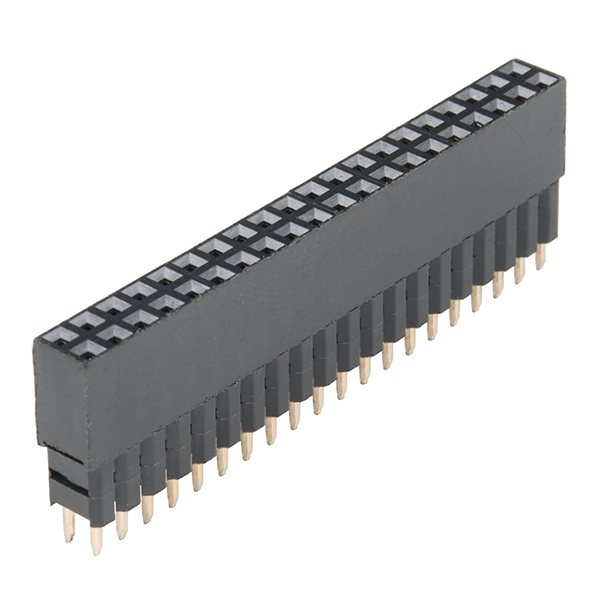
\includegraphics[width=0.5\textwidth,height=0.5\textheight,keepaspectratio]{female_gpio_headers.jpg}
			\caption{Female GPIO Headers, SparkFun Electronics (2016), Flickr, CC-BY 2.0}
			\label{fig:headers}
		\end{figure}

		Αφότου γίνει η κόλληση των Headers, μπορούν να χρησιμοποιηθούν τα αντίστοιχα καλώδια προκειμένου να συνδεθεί το Relay Module. Πρέπει ο χρήστης που θα το συνδέσει να συμβουλευτεί το διάγραμμα των GPIO Pins (γνωστό ως Pinout). Στο συγκεκριμένο παράδειγμα (\imgref{fig:rpi_to_relay}), έχει συνδεθεί στο GPIO Pin 18 (πράσινο καλώδιο). Για παροχή ρεύματος χρησιμοποιείται το 3V3 Pin (κόκκινο καλώδιο) και για Ground χρησιμοποιείται ένα από όλα τα GND Pins (μαύρο καλώδιο).

		\begin{figure}[h]
			\centering
				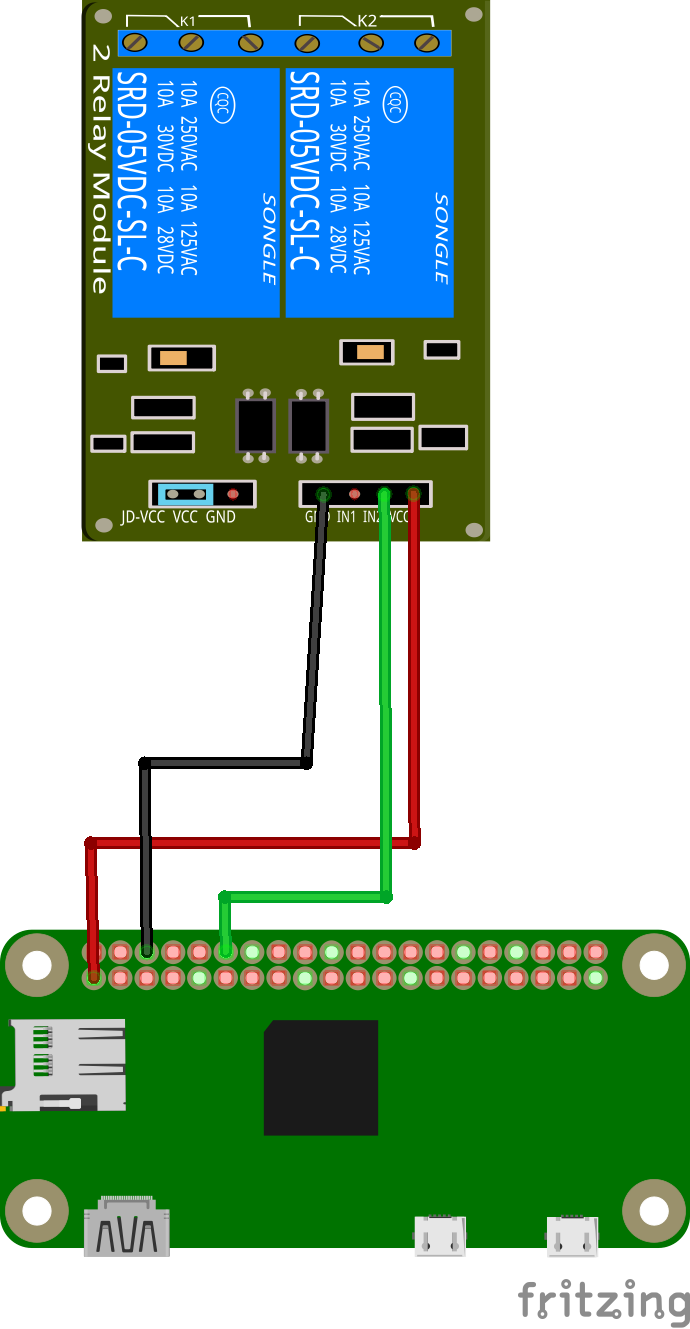
\includegraphics[width=0.5\textwidth,height=0.5\textheight,keepaspectratio]{rpi_to_relay.png}
			\caption{Σύνδεση ενός Raspberry Pi Zero W με ένα Relay Module}
			\label{fig:rpi_to_relay}
		\end{figure}


	\subsection{Σύνδεση με την χρήση Arduino}
		Αφότου γίνει Upload το Arduino Script που χρειάζεται για την λειτουργία του PiLock (βλ \fullref{sec:arduino_script}), μπορεί να γίνει σύνδεση του Arduino με το Relay. Το Relay Board μπορεί να συνδεθεί σε ένα από όλα τα Digital Pins του Arduino (πράσινο καλώδιο). Ρεύμα δίνεται μέσω του 5V Power Pin του Arduino και το Ground συνδέεται σε ένα εκ των τριών GND Pins του Arduino.